\section{INTRODUCTION}
\label{sec:introduction}

\subsection{Background and Motivation}

Optical communication infrastructure can support data transmission alongside
physical measurements, such as vibration along a fiber or receiver position
in a room \cite{OISAC_SCR00057,OISAC_SCR00196}.
Optical integrated sensing and communication (O-ISAC) uses this capability to
combine the two functions through shared infrastructure, hardware, or signals
\cite{OISAC_SCR00013,Mohsan2026OISACReview}.
This extends integrated sensing and communication (ISAC) to optical and
photonic systems \cite{Zhang2026ISACEvolution}.
ISAC is included among the usage scenarios in the International Mobile
Telecommunications framework for 2030 and beyond \cite{ITUR_M2160_2023}.
The opportunity to reuse resources brings a joint design problem, since their
operation must account for both communication and sensing requirements.

How these resources are shared depends on the signal path and the sensing
task. In fiber and optical wireless systems, light interacts with the sensing
medium or reaches the receiver or target
\cite{OISAC_SCR00013,OISAC_SCR00916,OISAC_SCR01085}.
In photonics-enabled wireless systems, optical components can generate the signal,
while propagation to the target occurs in the millimeter-wave or terahertz band
\cite{OISAC_SCR00036,OISAC_SCR00083}.
Figure~\ref{fig:oisac_platform_overview} illustrates these physical settings
and the resources used by both functions.
Its common design question is how choices of power and waveform, together
with timing and receiver design, affect communication and sensing performance.

\begin{figure*}[!t]
\centering
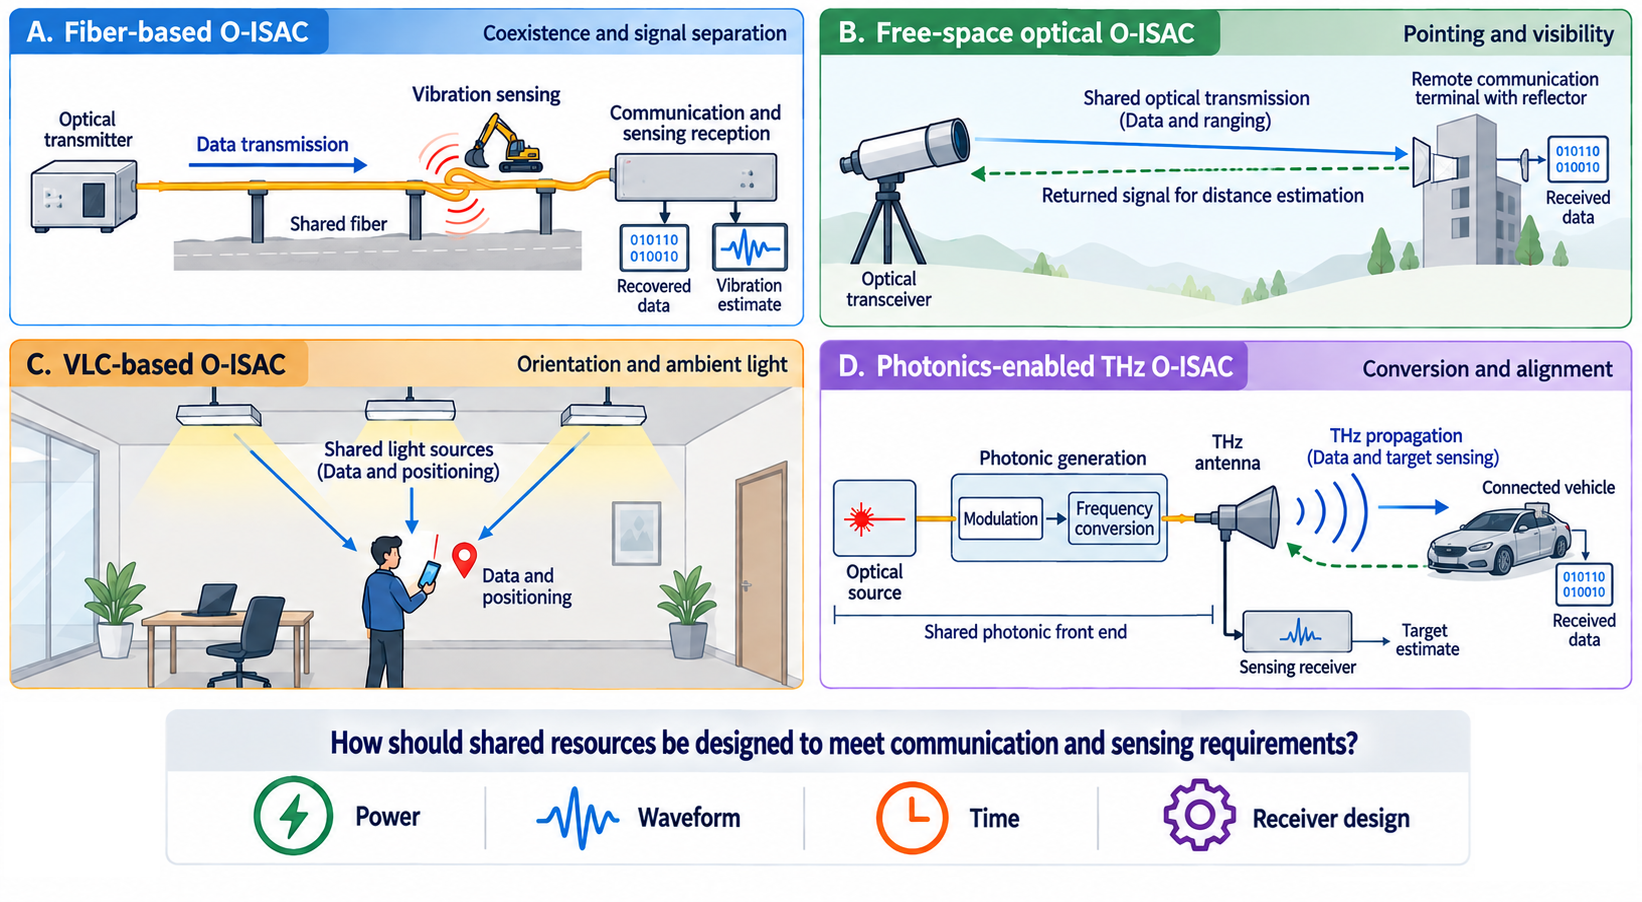
\includegraphics[width=\textwidth]{figures/fig_introduction_oisac_platforms.png}
\caption{Representative O-ISAC configurations in fiber, free-space optical,
visible-light, and photonics-enabled terahertz systems. Each panel identifies
a shared resource, the two functions it supports, and a representative physical
constraint. The lower panel highlights power and waveform choices alongside
timing and receiver design as common design considerations.}
\label{fig:oisac_platform_overview}
\end{figure*}

Shared operation can introduce a tradeoff or allow one function to assist the
other. In one fiber experiment, raising the sensing-probe power while holding
communication launch power fixed improved the sensing signal-to-noise ratio
but increased the communication bit error rate \cite{OISAC_SCR00057}.
In a visible-light prototype, position estimates guided beamforming toward the
receiver and improved the communication data rate at the tested locations
\cite{OISAC_SCR00196}.
The fiber result illustrates a power-dependent tradeoff, whereas the
visible-light result shows how sensing information can guide transmission.

A researcher selecting an O-ISAC approach needs to know which integration
mechanism fits the application and how it affects both functions.
Reported rates and sensing errors become useful for that choice when they
are linked to the shared design and its operating conditions.
These links can explain why a method is effective in one setting and what
must be tested before adapting it to another.
A synthesis of the literature should therefore connect physical architectures
to joint performance and to the experiments needed for further development.

\subsection{Related Surveys}
\label{sec:related_surveys}

Existing reviews provide several perspectives on these design questions,
through platform-specific analyses and broader views of O-ISAC. A tutorial on
optical architectures and waveform allocation
uses a common simulation setting to show communication error rate and ranging
error \cite{Wen2024OISACArchitectures}. A review of lighting, sensing, and
communication integration provides performance tables for visible-light and
hybrid systems \cite{Liang2024LiSACReview}. A waveform-focused review examines
photonic millimeter-wave and terahertz demonstrations and compares integrated
waveforms through models and experiments
\cite{Lyu2026PhotonicTHzWaveforms}. Other focused reviews address optical transmission and
estimation, or communication and sensing in fiber networks
\cite{Su2025OISACTheoryPractice,Khorasgani2026GeneralOpticalISACSurvey,
Liu2026OpticalFiberISACReview,Lu2026ConvergedFiberISACReview}.

Broader surveys connect these technical developments to larger research
questions. An evolution-oriented survey traces ISAC across spectrum, network
scale, and sensing modalities, including optical and RF--optical systems
\cite{Zhang2026ISACEvolution}. A broad O-ISAC review brings together optical
platforms, experimental results, waveform design, and applications
\cite{Mohsan2026OISACReview}. These two surveys also discuss performance
measures and the need for further evaluation.
Together, these works explain design choices, report numerical
demonstrations, and identify research directions.

Table~\ref{tab:prior_surveys} distinguishes the physical coverage and review
approach of representative works. Its platform columns identify where the
sensing interaction takes place. The last two columns address how studies
are selected and how results from different studies are judged comparable.
This distinction matters because a controlled waveform comparison and a
comparison between independently reported experiments answer different
questions. The latter also requires agreement on what was measured and under
which conditions.

\begin{table*}[!t]
\caption{Physical coverage and review approach of representative related
reviews and tutorial-style syntheses}
\label{tab:prior_surveys}
\centering
\begingroup
\footnotesize
% Local Wasy glyphs keep the full and half-filled circles the same size.
\newcommand{\surveyGlyph}[1]{{\fontencoding{U}\fontfamily{wasy}\selectfont\char#1}}
\newcommand{\surveyFull}{\mbox{\surveyGlyph{32}}}
\newcommand{\surveyPartial}{\leavevmode
  \hbox to 0pt{\surveyGlyph{71}\hss}\hbox{\surveyGlyph{35}}}
\setlength{\tabcolsep}{3.5pt}
\renewcommand{\arraystretch}{1.2}
\renewcommand{\tabularxcolumn}[1]{m{#1}}
\begin{tabularx}{\textwidth}{@{}%
>{\raggedright\arraybackslash}m{0.13\textwidth}
>{\raggedright\arraybackslash}m{0.30\textwidth}
>{\centering\arraybackslash}m{0.055\textwidth}
>{\centering\arraybackslash}m{0.09\textwidth}
>{\centering\arraybackslash}m{0.09\textwidth}
>{\centering\arraybackslash}X
>{\centering\arraybackslash}X@{}}
\toprule
\textbf{Ref. / year} & \textbf{Main focus} &
\multicolumn{3}{c}{\textbf{Optical platforms}} &
\multicolumn{2}{c}{\textbf{Review approach}} \\
\cmidrule(lr){3-5}\cmidrule(l){6-7}
& & Fiber & Optical wireless & Photonic wireless &
Study selection & Cross-study comparison rules \\
\midrule
\cite{Wen2024OISACArchitectures} (2024) &
Optical architectures, waveform design, and resource allocation &
\textemdash & \surveyFull & \textemdash & \textemdash & \textemdash \\
\addlinespace[3pt]
\cite{Liang2024LiSACReview} (2024) &
Lighting--sensing--communication integration and hybrid links &
\textemdash & \surveyFull & \textemdash & \textemdash & \textemdash \\
\addlinespace[3pt]
\cite{Lyu2026PhotonicTHzWaveforms} (2026) &
Integrated photonic waveforms and controlled performance comparisons &
\textemdash & \textemdash & \surveyFull & \textemdash & \textemdash \\
\addlinespace[3pt]
\cite{Zhang2026ISACEvolution} (2026) &
ISAC evolution across spectrum, networks, and sensing modalities &
\surveyPartial & \surveyFull & \surveyFull & \textemdash & \surveyPartial \\
\addlinespace[3pt]
\cite{Mohsan2026OISACReview} (2026) &
Optical platforms, experimental demonstrations, and applications &
\surveyFull & \surveyFull & \surveyFull & \textemdash & \surveyPartial \\
\midrule
\textbf{This survey} &
Shared-resource performance relations and evidence-based evaluation &
\surveyFull & \surveyFull & \surveyFull & \surveyFull & \surveyFull \\
\bottomrule
\end{tabularx}
\par\vspace{4pt}
\noindent
\parbox{\textwidth}{\raggedright\footnotesize
\surveyFull: structured treatment; \surveyPartial: selected discussion or an
identified research need; \textemdash: not developed in the stated sense.
Fiber denotes sensing in the fiber, not fiber transport alone; photonic
wireless denotes optically generated or processed signals with wireless
RF propagation. Only optical-related coverage is marked for
\cite{Zhang2026ISACEvolution}.
Study selection denotes an explicit search and eligibility procedure.
Cross-study comparison rules address metric definitions, measurement points,
conditions, baselines, and supporting evidence; they are distinct from a
controlled comparison within one model or experiment.\par}
\endgroup
\end{table*}

A further need is to explain when a reported result can guide another
design. The difficulty of using common performance measures across RF and
optical systems is discussed in \cite{Zhang2026ISACEvolution}, while shared
benchmarks are identified as a research need in \cite{Mohsan2026OISACReview}.
These observations motivate comparison rules that connect shared design
choices to both performance outcomes and specify the measurement conditions
under which results can be compared.

\subsection{Scope and Contributions}

This survey examines O-ISAC in guided optical systems, optical wireless links,
and photonics-enabled wireless systems, including hybrid configurations.
We analyze how shared infrastructure, signals, and design objectives connect
communication and sensing, and how these connections shape joint performance.

The contributions address physical integration, performance interpretation,
and experimental evaluation.
\begin{itemize}
\item \textbf{A physical basis for selecting an O-ISAC design.}
We distinguish platforms by their sensing paths and identify how hardware,
signals, and allocated resources connect the two functions. This explains
which integration mechanisms fit a given physical setting and which
constraints must be considered when adapting them
(Sections~\ref{sec:foundations_comparison}
and~\ref{sec:optical_modality_families}).

\item \textbf{A common basis for interpreting performance.}
We relate waveform and receiver choices, together with resource allocation,
to communication rate and reliability alongside sensing accuracy and
resolution. We distinguish relationships demonstrated within a study from
comparisons that require compatible metrics, measurement points, and
operating conditions
(Sections~\ref{sec:foundations_comparison} and~\ref{sec:tradeoffs}).

\item \textbf{Evaluation priorities derived from the evidence.}
We derive joint tests from the validation limits observed across optical
platforms. These tests pair communication and sensing measurements with
separate-function baselines under changes in traffic, propagation conditions,
or hardware stability
(Sections~\ref{sec:validation_reproducibility}
and~\ref{sec:discussion_roadmap}).
\end{itemize}

Section~\ref{sec:foundations_comparison} introduces the physical and performance
concepts used in the review, and Section~\ref{sec:review_methods} describes the
review methods. Sections~\ref{sec:optical_modality_families}
through~\ref{sec:technologies_applications_6g} examine platforms, joint design,
validation, and applications. Section~\ref{sec:discussion_roadmap} develops the
research priorities, and Section~\ref{sec:conclusion} concludes the article.

\FloatBarrier
